% Twenty Seconds Resume/CV
% LaTeX Template
% Version 1.0 (14/7/16)
%
% Original author:
% Carmine Spagnuolo (cspagnuolo@unisa.it) with major modifications by 
% Vel (vel@LaTeXTemplates.com) and Harsh (harsh.gadgil@gmail.com)
%
% License:
% The MIT License (see included LICENSE file)
%
%%%%%%%%%%%%%%%%%%%%%%%%%%%%%%%%%%%%%%%%%

%----------------------------------------------------------------------------------------
%	PACKAGES AND OTHER DOCUMENT CONFIGURATIONS
%----------------------------------------------------------------------------------------
%INCLUDE ALL THE DATAS TO RUN THE PRODUCTION
\newcommand{\fromName}{Daniel Schmid}
\newcommand{\fromStreet}{Pergolastrasse 4}
\newcommand{\fromPlz}{3185}
\newcommand{\fromPlaceName}{Schmitten}
\newcommand{\fromPlace}{\fromPlz \hspace{1pt} \fromPlaceName}
\newcommand{\fromAdress}{ \fromName \\ \fromStreet \\ \fromPlace}
\newcommand{\fromDate}{\fromPlaceName, \today}
\newcommand{\fromTel}[1][078 771 55 22]{Tel: #1}
\newcommand{\wiesoich}{
\textbf{Meine} praxiserprobten Kenntnisse in der Software-Entwicklung in C\#.Net, 
sowie meine langjährige Erfahrung in der\\ Analyse, Konzeption, Umsetzung und dem
Testing individueller Lösungen, bringe ich ein fundiertes und \\praxiserprobtes
Know-How mit.

\textbf{Durch} meinen ausgeprägten und \\vielseitigen technischen Hintergrund,\\ meiner
Kommunikationsfähigkeit und durch meine hohe Dienstleistungsmentalität
kann ich im bestehenden Team, schnell \\ einen Mehrwert generieren.
}


\newcommand{\toName}{SRF Studio Zürich \\ Frau Junker }
\newcommand{\toStreet}{ Fernsehstrasse 1 - 4 }
\newcommand{\toPlace}{8052 Zürich }
\newcommand{\toAdress}{ \toname  \\ \tostreet \\ \toplace}
\newcommand{\letterSubject}{Bewerbung als Fachverantwortlicher Digital Analytics }
\newcommand{\toContact}{Sehr geehrte Damen}
\newcommand{\letterText}{
Als erfahrener Softwareentwickler betrachte ich Analyse als Schlüssel zum Erfolg. Wie aus
meinem Lebenslauf hervorgeht, gewinnen Sie mit mir einen kundenorientierten Analytiker mit
raschem Auffassungsvermögen, Teamgeist und hoher Einsatzbereitschaft. \\\\
Dank meiner zuverlässigen und innovativen Arbeitsweise gelang
es mir stets, neue Themengebiete schnell zu erschliessen. So konnte ich in
verschiedenen Projekten meine fachlichen Kompetenzen erfolgreich unter Beweis stellen. Durch meine langjährige Berufspraxis habe ich gelernt, dass dieser Beruf ohne ein gewisses
Mass an Kreativität und Geduld nicht durchführbar ist. Zusammen mit meinem Team konnte
ich verschiedenste Probleme aller Entwicklungsebenen erfolgreich lösen und stets eine sehr
hohe Kundenzufriedenheit aufweisen.\\\\
Es begeistert mich zudem für das SRF meinen Beitrag zum Erfolg leisten zu dürfen und
meine eigene Erfolgsgeschichte, langfristig in Ihrem Unternehmen fortzusetzen. Ich kann mich
in einem neuen Umfeld gut einbringen und lerne schnell, mit neuen Arbeitsweisen vertraut zu
werden. Mit hektischen Situationen kann ich gut umgehen und bewahre stets einen kühlen
Kopf.\\\\
Ich freue mich auf Ihre Rückmeldung und überzeuge Sie gerne in einem persönlichen
Vorstellungsgespräch von meiner Motivation.
Bei Fragen stehe ich Ihnen gerne zur Verfügung.
}




\documentclass[a4paper]{twentysecondcv} % a4paper for A4

% Command for printing skill overview bubbles
\newcommand\skills{ 
~
	\smartdiagram[bubble diagram]{
        \textbf{~~~~Daniel~~~~}\\\textbf{~~~~Schmid~~~~},
        \textbf{~~~~~~~~ruhig~~~~~~~~},
        \textbf{pragmatisch},
        \textbf{~~Teamgeist~~},
        \textbf{~~~~~kreativ~~~~~},
        \textbf{~analytisch~},
        \textbf{~ziel~} - \\\textbf{~~orientiert~~}
    }
}

% Programming skill bars
\programming{{C $\textbullet$ C++  $\textbullet$ \LaTeX $\textbullet$ Java / 2.5}, { PHP $\textbullet$ Bash $\textbullet$ PowerShell  / 3.5}, {HTML5 $\textbullet$ SASS $\textbullet$  / 4},{C\#.Net $\textbullet$ MSSQL $\textbullet$ JS $\textbullet$ / 5}}

% Projects text
\projects{
\wiesoich
}

%----------------------------------------------------------------------------------------
%	 PERSONAL INFORMATION
%----------------------------------------------------------------------------------------
% If you don't need one or more of the below, just remove the content leaving the command, e.g. \cvnumberphone{}

\cvname{\fromName} % Your name
\cvjobtitle{ Full Stack Entwickler } % Job
% title/career

\cvlinkedin{/in/schmid-daniel/}
\cvgithub{}
\cvnumberphone{078 771 55 22} % Phone number
%\cvsite{daenu-schmid.ch} % Personal website
\cvsite{}
\cvmail{daenu.schmid@gmail.com} % Email address

%----------------------------------------------------------------------------------------

\begin{document}

\includepdf[pages={1},scale=1]{out/business2.pdf}

\makeprofile % Print the sidebar
\hypertarget{work_back}{}
\section{Berufliche Tätigkeit}
\begin{twenty}
	\twentyitem
    	{seit 2010}
        {}
        {Link Institut AG \textnormal{Luzern}}
        {\hyperlink{link}{\textcolor{pblue}{Zwischenzeugnis}}}
        {Spezialist IT Entwicklung}
        {\begin{itemize}
\item Realisierung von Projekten bzw. Teilmodulen im C\# .NET-Umfeld
(Web-Applikation, Desktop-Applikationen)
\item Selbständige Konzeption und Entwicklung von kleinen bis
mittleren Anwendungen im Bereich „Online-Marktforschung"
\item Mitarbeit bei der Datenpflege und Wartung des LINK Internet-
Panels und Hauptverantwortung für einzelne Anwendungen
\item Weiterentwicklung und Wartung bestehender Anwendungen im
C\# .NET-Umfeld
\item Allgemeine Wartungsaufgaben (MS-SQL Datenbanken,
Anwendungen)
\item Studienspezifische Entwicklungen komplexer Online-
Befragungen
\item Mithilfe beim Aufbau und Organisation der
Entwicklungsumgebung
\item Aufbau und Unterhalt SVN \// GIT
	\end{itemize}}		
	\twentyitem
    	{}
        {}
        {}
        {}
        {}
        {}
	\twentyitem
    	{2009 - 2010}
        {}
        {Datahouse AG \textnormal{Zürich}}
        {\hyperlink{datahouse}{\textcolor{pblue}{Arbeitszeugnis}}}
        {Applikationsentwickler}
        {
		\begin{itemize}
		\item Entwicklung von Webapplikationen in PHP
		\item Implementation von SOAP-Web-Services in C++
		\item Erstellung verschiedener Templates in \LaTeX
		\end{itemize}
	}	
	\twentyitem
    	{}
        {}
        {}
        {}
        {}
        {}
	\twentyitem
    	{2008 - 2009}
        {}
        {Jordi AG \textnormal{Schlieren}}
        {\hyperlink{jordi}{\textcolor{pblue}{Arbeitszeugnis}}}
        {Bereich: Mikroprozessorprogrammierung}
        {}
	\twentyitem
    	{2006 - 2007}
        {}
        {T-Systems Schweiz AG \textnormal{Zollikofen}}
        {\hyperlink{tsystems}{\textcolor{pblue}{Arbeitszeugnis}}}
        {}
        {}
	\twentyitem
    	{2005}
        {}
        {Bundesamt für Sozialversicherung \textnormal{Bern}}
        {\hyperlink{bsv}{\textcolor{pblue}{Arbeitszeugnis}}}
        {Berufspraktikum als Sachbearbeiter}
        {}

	\twentyitem
    	{2004}
	{}
        {Booktrading,\textnormal{Freiburg}}
        {\hyperlink{booktrading}{\textcolor{pblue}{Arbeitszeugnis}}}
        {Berufspraktikum als Sachbearbeiter Buchhaltung}
	{}
	\twentyitem
    	{2003}
	{}
        {WABCO (Schweiz) GmbH \textnormal{Bern Bümpliz}}
        {\hyperlink{wabco}{\textcolor{pblue}{Lehr - und Arbeitszeugnis}}}
        {Sachbearbeiter Betriebsbuchhaltung/Reporting}
	{}	
\end{twenty}
%----------------------------------------------------------------------------------------
%	 EDUCATION
%----------------------------------------------------------------------------------------
\hypertarget{cert_back}{}
\section{Ausbildung}
\begin{twenty} % Environment for a list with descriptions
	\twentyitem
    	{seit 2019}
        {}
        {MCSA Lehrgang \textnormal{Zürich}}
        {}
        {}
        {}	
	\twentyitem
    	{2007 - 2009}
	{}
        {Informatikumschulung}
        {\hyperlink{informatik}{\textcolor{pblue}{Diplom}}}
        {Fachrichtung Applikationsentwicklung}
        {}
	\twentyitem
    	{2005}
	{}
        {Cobol Programmierkurs \textnormal{Zürich}}
        {\hyperlink{cobol}{\textcolor{pblue}{Zertifikat}}}
        {}
        {}
	\twentyitem
    	{2004}
	{}
        {Englischintensivkurs beim WSI \textnormal{Freiburg}}
        {\hyperlink{toeic}{\textcolor{pblue}{Zertifikat}}}
        {}
        {}
	\twentyitem
    	{2000 - 2003}
        {}
        {Wirtschafts- und Kaderschule \textnormal{KV Bern}}
        {\hyperlink{kv}{\textcolor{pblue}{Diplom}}}
        {}
        {}
\twentyitem
    	{2000 - 2003}
	{}
        {WABCO (Schweiz) GmbH \textnormal{Bern Bümpliz}}
        {}
        {Kaufmännische Lehre}
	{}	%\twentyitem{<dates>}{<title>}{<organization>}{<location>}{<description>}
\end{twenty}
%----------------------------------------------------------------------------------------
%	 EXPERIENCE
%----------------------------------------------------------------------------------------

\section{Referenzen}

\begin{twenty} % Environment for a list with descriptions
\twentyitem
    	{auf Anfrage}
	{}
        {}
        {}
        {}
        {}
	%\twentyitem{<dates>}{<title>}{<location>}{<description>}
\end{twenty}
\newpage
\hypertarget{link}{}

\includepdf[pages={1},scale=1,%
	picturecommand*={%
	\put(16,800){\hyperlink{work_back}{\textcolor{pblue}{zurück}}}%
}]{cert/2019_link.pdf}

\hypertarget{datahouse}{}

\includepdf[pages={1},scale=1,%
	picturecommand*={%
	\put(16,800){\hyperlink{work_back}{\textcolor{pblue}{zurück}}}%
}]{cert/10_datahouse.pdf}
\hypertarget{jordi}{}

\includepdf[pages={1},scale=1,%
	picturecommand*={%
	\put(16,800){\hyperlink{work_back}{\textcolor{pblue}{zurück}}}%
}]{cert/09_jordi_ag.pdf}
\hypertarget{tsystems}{}

\includepdf[pages={1},scale=1,%
	picturecommand*={%
	\put(16,800){\hyperlink{work_back}{\textcolor{pblue}{zurück}}}%
}]{cert/07_t_systems.pdf}
\hypertarget{bsv}{}

\includepdf[pages={1},scale=1,%
	picturecommand*={%
	\put(16,800){\hyperlink{work_back}{\textcolor{pblue}{zurück}}}%
}]{cert/05_bsv.pdf}

\includepdf[pages={2},scale=1]{cert/05_bsv.pdf}
\hypertarget{booktrading}{}

\includepdf[pages={1},scale=1,%
	picturecommand*={%
	\put(16,800){\hyperlink{work_back}{\textcolor{pblue}{zurück}}}%
}]{cert/04_booktrading.pdf}
\hypertarget{wabco}{}

\includepdf[pages={1},scale=1,%
	picturecommand*={%
	\put(16,800){\hyperlink{work_back}{\textcolor{pblue}{zurück}}}%
}]{cert/03_wabco-crop.pdf}
\hypertarget{informatik}{}

\includepdf[pages={1},scale=1,%
	picturecommand*={%
	\put(16,800){\hyperlink{cert_back}{\textcolor{pblue}{zurück}}}%
}]{cert/09_informatiker.pdf}

\includepdf[pages={1},scale=1,%
	picturecommand*={%
	\put(16,800){\hyperlink{cert_back}{\textcolor{pblue}{zurück}}}%
}]{cert/09_cert_informatik.pdf}
\hypertarget{cobol}{}
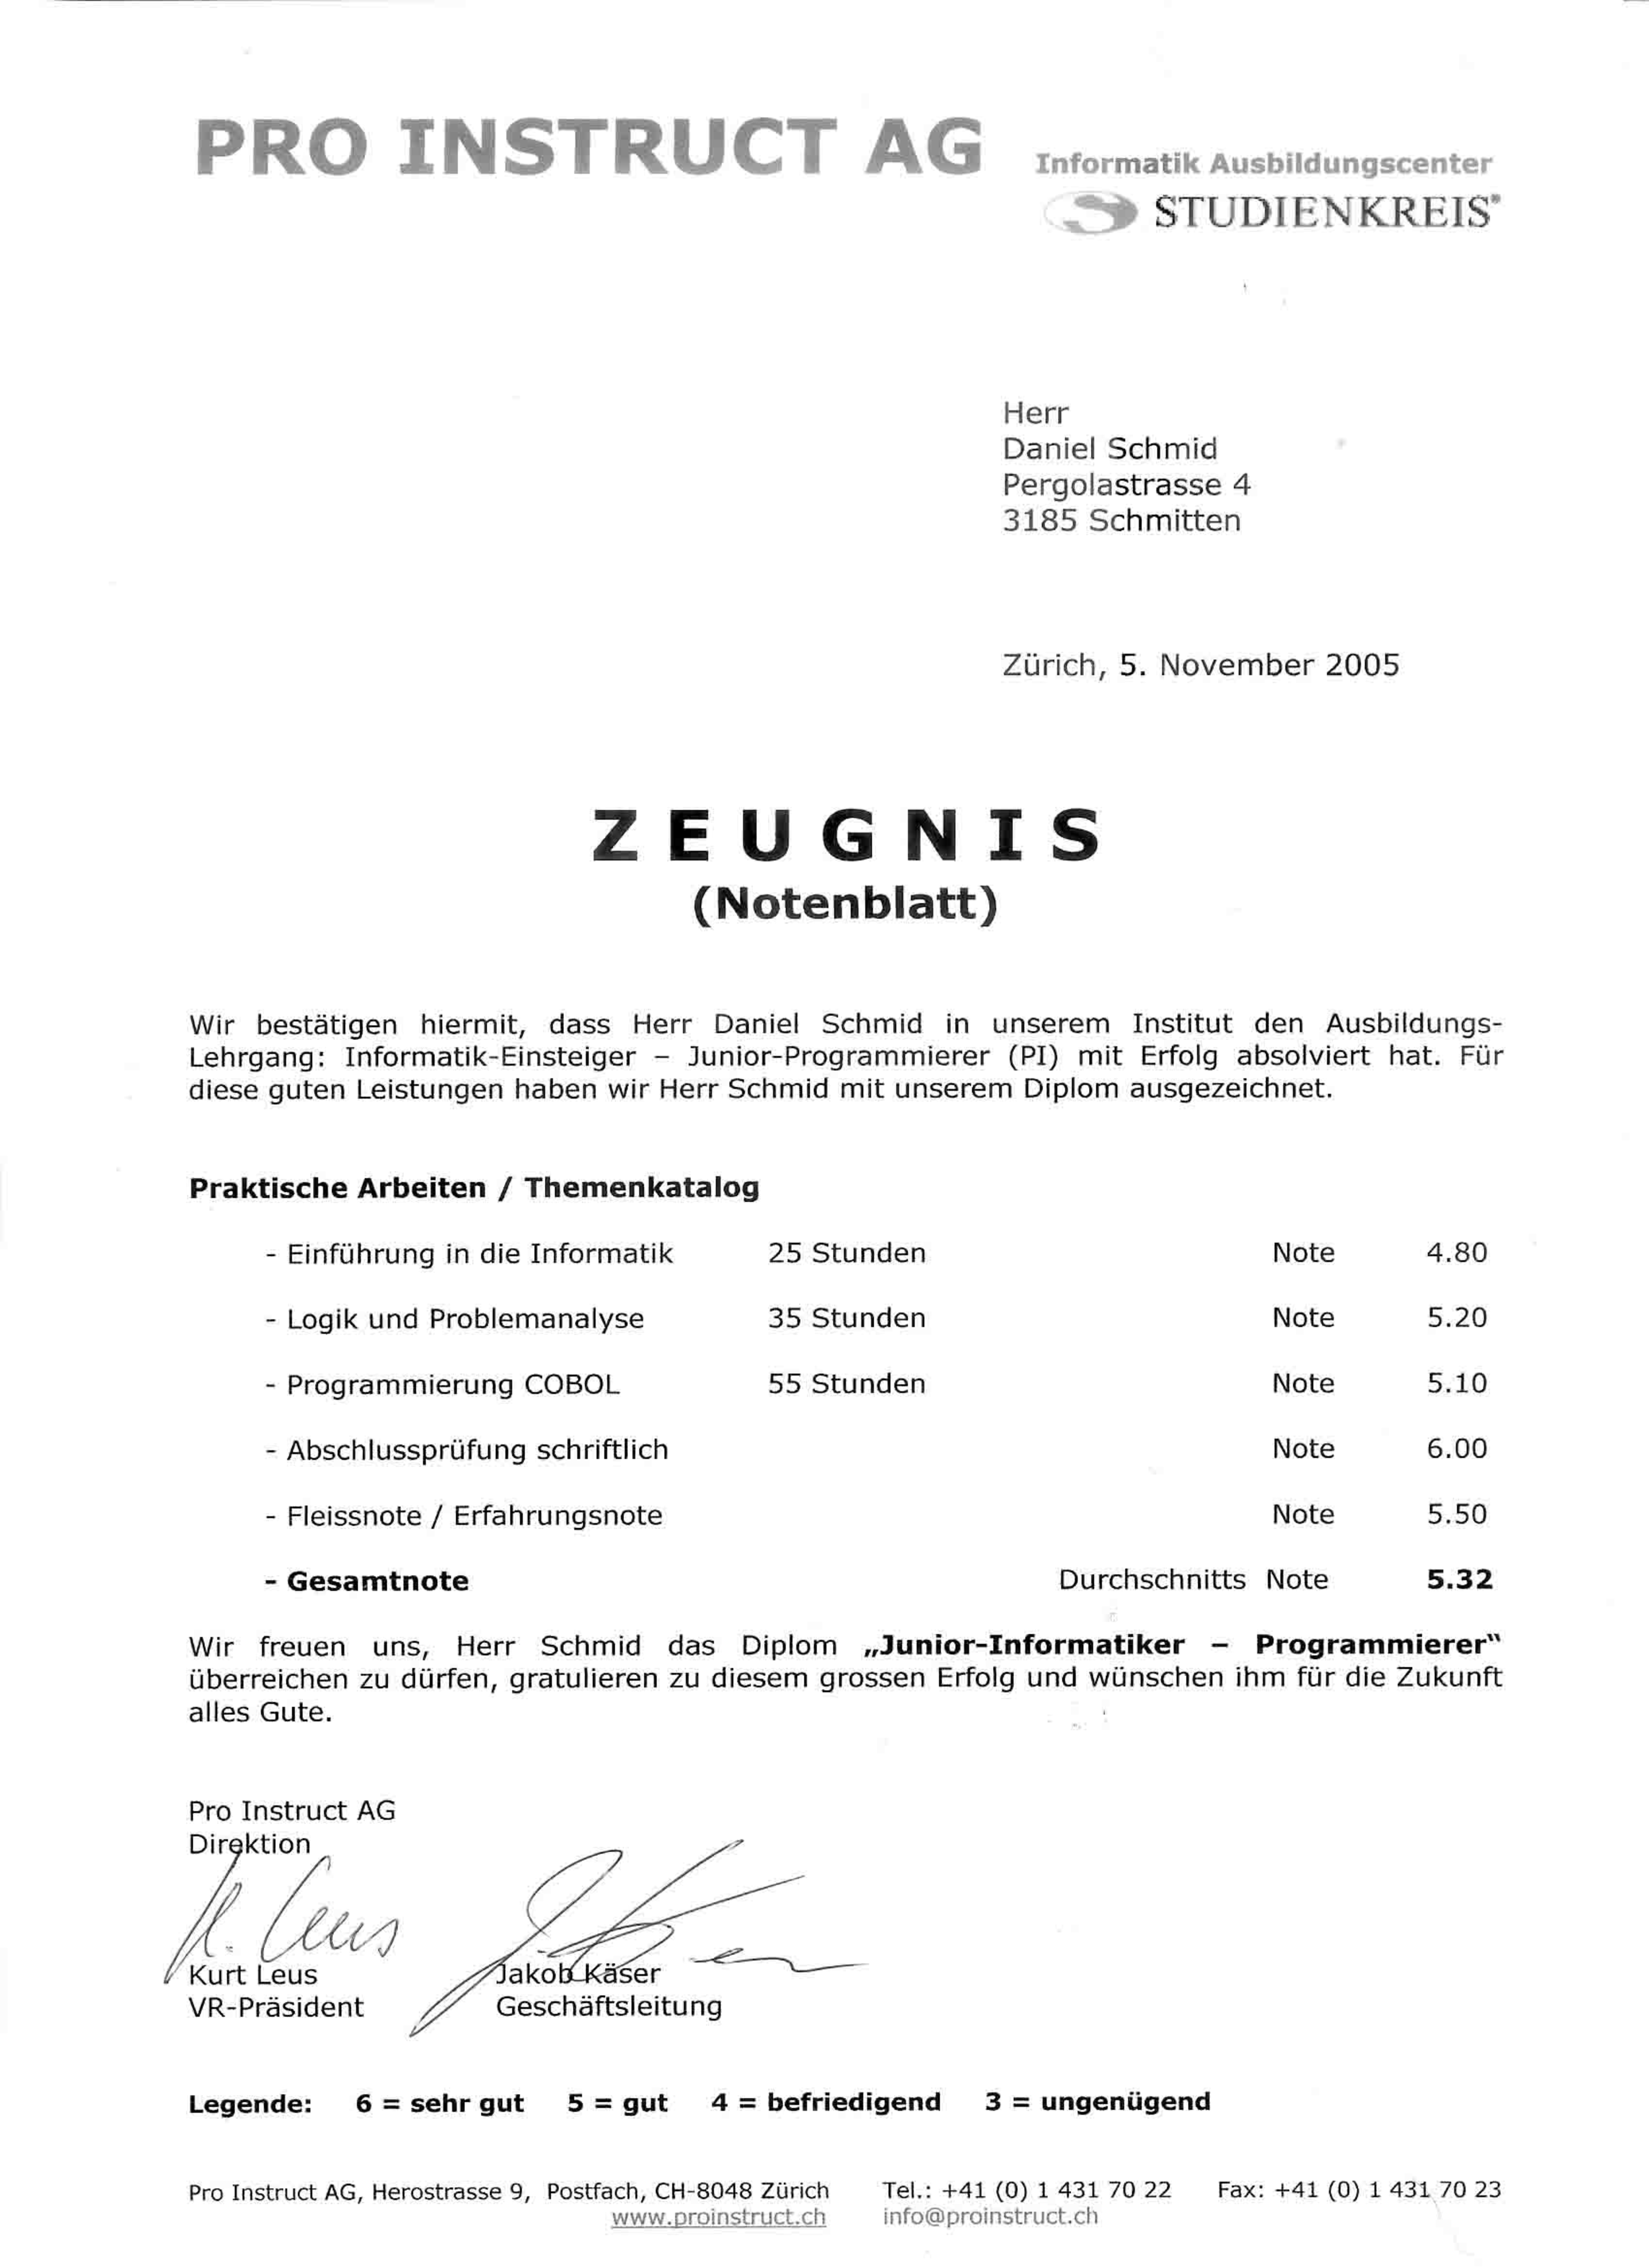
\includepdf[pages={1},scale=1,%
	picturecommand*={%
	\put(16,800){\hyperlink{cert_back}{\textcolor{pblue}{zurück}}}%
}]{cert/05_course_cobol.pdf}
\hypertarget{toeic}{}

\includepdf[pages={1},scale=1,%
	picturecommand*={%
	\put(16,800){\hyperlink{cert_back}{\textcolor{pblue}{zurück}}}%
}]{cert/05_toeic.pdf}
\hypertarget{kv}{}

\includepdf[pages={1},scale=1,%
	picturecommand*={%
	\put(16,800){\hyperlink{cert_back}{\textcolor{pblue}{zurück}}}%
}]{cert/03_cert_kv.pdf}
%\hypertarget{siz}{}
%
\includepdf[pages={1},scale=1,%
%	picturecommand*={%
%	\put(16,800){\hyperlink{cert_back}{\textcolor{pblue}{zurück}}}%
%}]{cert/02_course_siz.pdf}
\end{document} 
